\section{Funcions seleccionades per a la Web}
\subsection{Comptes d'usuari}

\begin{figure}[htpb!]
    \centering
    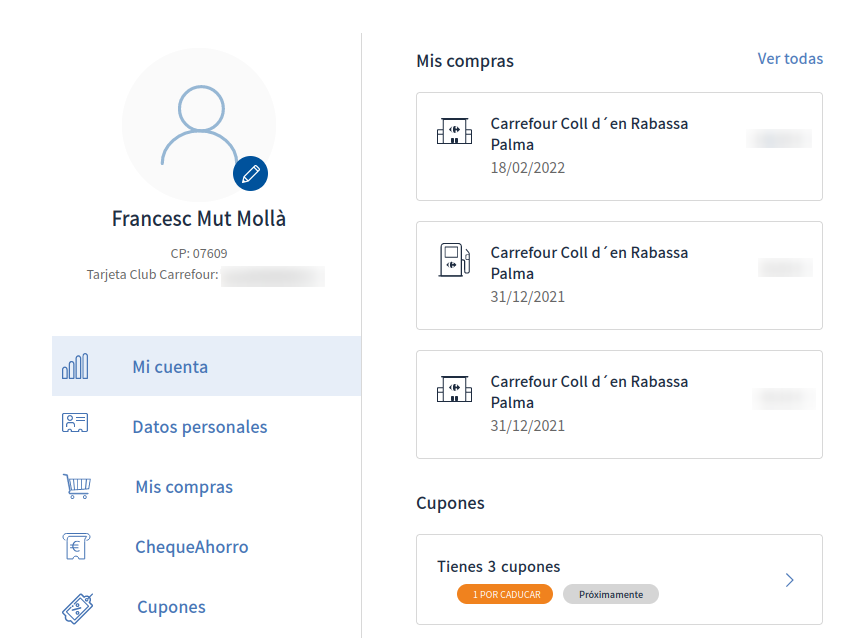
\includegraphics[width=400pt]{figures/Usuaris.png}
\end{figure}

    Com podem veure a la foto, a la pàgina web necessitarem una secció de Mis Compras on guardar un registre de 
    tots els nostres pedidos, i dins Datos Personales nosaltres hem guardat el correu, nom complet, adreça on 
    enviar les compres i mètode de pagament.
    
    \textbf{Un usuari pot fer més d'una compra}, però el més segur es que mai siguin suficients per a superar el límit 
    d'un document incrustat, per tant, per aquesta \textbf{relació 1:F emprarem un document incrustat dins cada Usuari.}

    Els \textbf{pedidos i els envíos seràn una relació F a 1, refferencing}, ja que considerem que cada pedido està 
    relacionat a una (o més) adreces d'origen i una única adreça destí, ja que la pàgina del Carrefour et permet triar 
    la direcció d'origen preferida (En la foto, Carrefour Coll de'n Rabassa), i depenent de disponibilitat pot ésser 
    que ens enviin productes des de dues ubicacions diferents, com per exemple el Carrefour del Coll i el seu magatzem del polígon.

\newpage

\subsection{Processament de comandes}

\begin{figure}[htpb!]
    \centering
    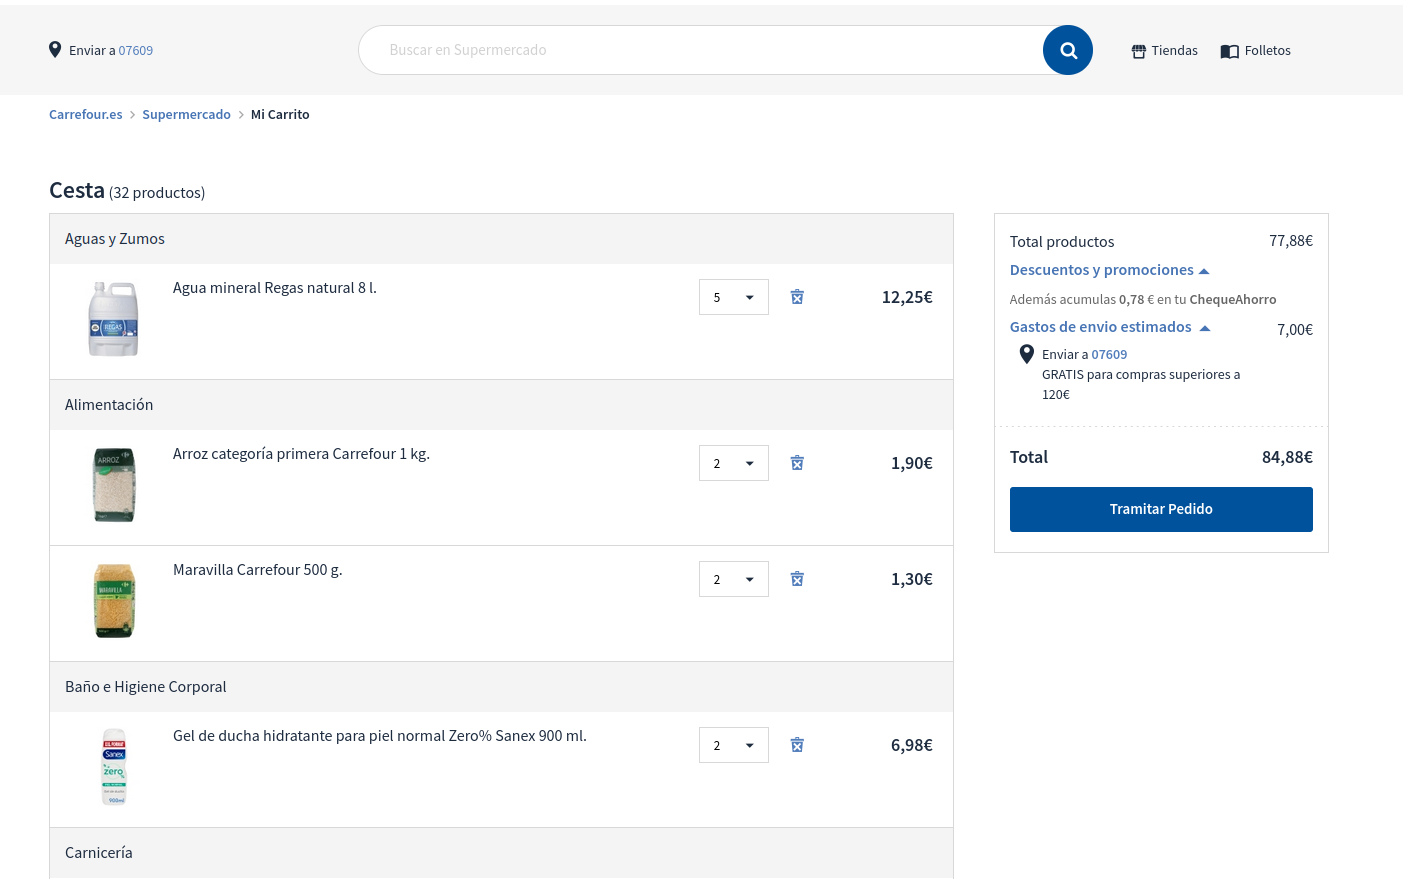
\includegraphics[width=400pt]{figures/Pedido.png}
\end{figure}

A la pàgina de processament de comandes, com podem veure, diferenciam els productes per seccions, per tant, necessitarem
que la col·lecció de comandes tingui els seguents apartats:

\begin{enumerate}
    \item Array de productes, on referenciarem els productes i les seves dades (com preu i categoria)
    \item Array de documents d'envíos, amb tota la info i el seguiment.
    \item Subtotal de la compra
    \item Data de la compra
    \item Array de tendes des de les quals prepararem els productes per ser enviats.
\end{enumerate}

Un cop completa aquesta llista de la compra l'usuari tramita la comanda i afegeix la seva informació de pagament, 
que es guarda en un array a la col·lecció d'usuaris. Aquí l'usuari pot modificar també la seva adreça.

A partir del subtotal es calcula un descompte que es guardarà a la array de mètodes de pagament de l'usuari.

\newpage 

\subsection{Categories i productes}

\begin{figure}[htpb!]
    \centering
    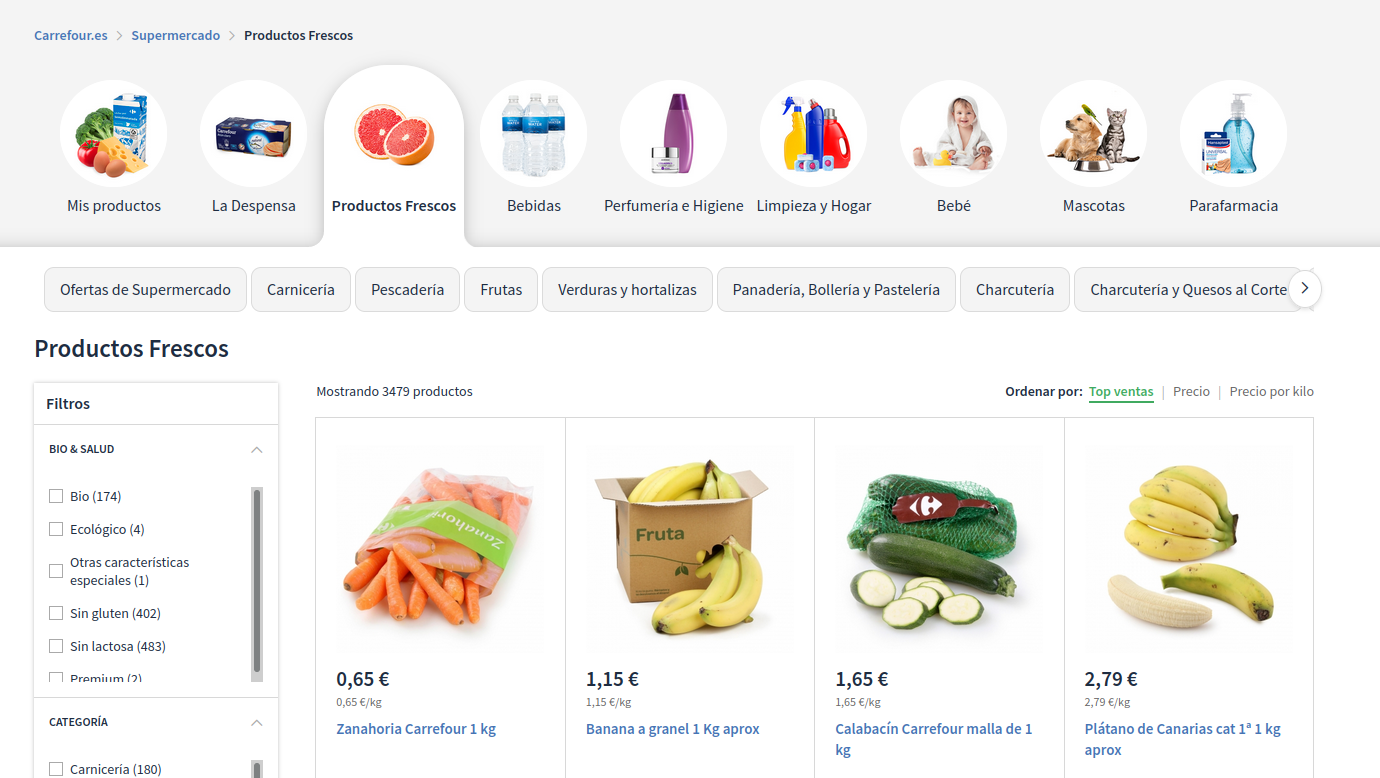
\includegraphics[width=400pt]{figures/Productes.png}
\end{figure}

Els productes es poden organitzar mitjançant categories (frescos, begudes, carns) i tipus (bio, premium, sense lactosa), 
i filtrar segons al·lèrgens.

\subsection{Logística}

La logística de les comandes per web del Carrefour és complexa. Per començar, cada comanda tindrà
un o n enviaments, dependrà dels productes disponibles a cada tenda o magatzem.

Per tant, cada enviament serà un document incrustat a una comanda, que contindrà:

\begin{itemize}
    \item El nom de l'empresa que gestiona l'enviament
    \item Les dades de l'usuari que ho ha de rebre. (nom i adreça)
    \item L'adreça de la tenda on ha de fer la recollida
    \item Informació de control de l'enviament (data d'entrega prevista, data de procés i data de recollida.)
\end{itemize}